\label{calibration}
%\subsection{Calibration}
The design of the calibration system for DUNE-PT pursues two principal goals. The first is to calibrate the detector itself to
provide high quality data for successive data analysis and the second is to test and optimize the calibration tools themselves for future
use in the DUNE far detectors.

The accuracy of track and kinematics reconstruction and particle identification largely relies on the knowledge of the electric field map, purity map, and temperature inside the active detector volume. The electric field in the drift region, designed to be a uniform 500 V/cm, could vary at different locations due to sagged wires, misalignment and imperfections in the field cage. 


The electric field could also be distorted by the space charge.  Electrons and ions which are generated by the passing of high energy particles drift in opposite directions to anode and cathode planes, respectively. The electrons drift at about 1.6 mm/$\mu s$ and take 2.25 ms to travel the maximum distance between APAs and CPAs. The ions, drifting at $\sim$ 8$\times 10^{-6}$~mm/$\mu s$, can take up to 7.5 minutes to travel the same distance. \\
The surface cosmic ray flux entering the detector imposes a large space-charge effect to the detector. 
%The magnitude of the distortion of the electric field is expected to be on the same order as the microBooNE detector which is also on the surface.  An example of the electric field distortion simulated in the microBooNE detector is shown in Fig.~\ref{fig:space_charge}.
%\begin{figure}[h!]
%  \centering
%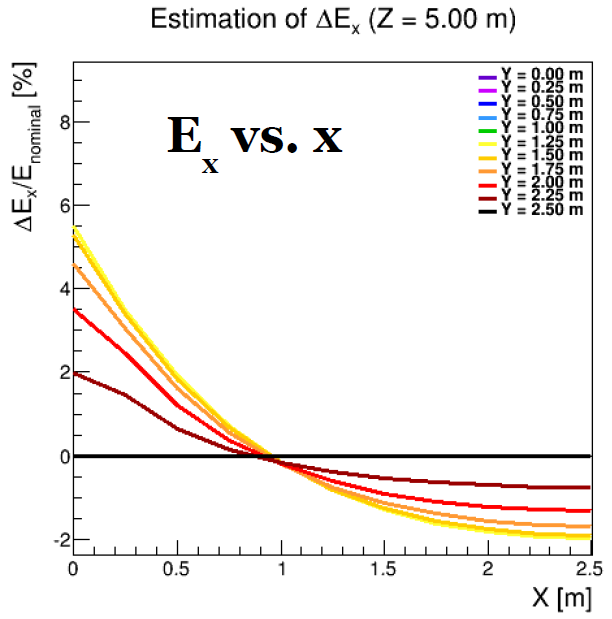
\includegraphics[width=0.49\textwidth,height=6.0cm]{figures/spacechargeEvsx} 
%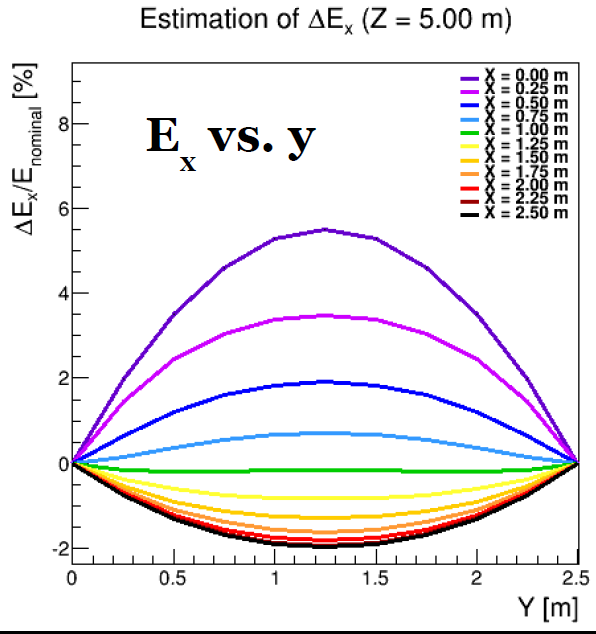
\includegraphics[width=0.49\textwidth,height=6.0cm]{figures/spacechargeEvsy} 
%  \caption{Fractional deviation of the microBooNE drift field $E_{x}$ as a function of position due to space charge effects.  The figure on the left shows the variation as a function of the distance between the cathode (x = 0) and the anode (x = 2.5 m).  The figure on the right shows the variation as a function of the vertical position.  The plots are from \cite{ref:space_charge}.
%{\color{red}  combine e+e-, improve information content (y-axis, change colors, etc )
%}
%}
%\label{fig:space_charge}
%\end{figure}
Distortion of the electric field could result in centimeter levels of uncertainty in position reconstruction and can also make a difference in electron-ion recombination and light output. 

The temperature of liquid argon affects the electron drift velocity and has a gradient of about -1.9\%/K. Precision measurement of temperature could be easily achieved with commercial silicon diode sensors down to tens of milliKelvin. 

Purity of argon directly affects the amount of surviving electrons, which would be used to estimate the amount of energy deposited in that wire space. This energy deposition, dE/dx, is a key quantity for particle identification. Monitoring argon purity is also essential for the operation of the experiment.

Multiple means should be employed to measure the electric field, the purity of liquid argon and its temperature. 
The presently foreseen calibration equipment includes:
\begin{itemize}
\item Gas purity analyzers
\item Liquid purity monitors
\item Temperature sensors
\item Laser calibration system
\item Muon detector system
\end{itemize}

The gas purity analyzers for oxygen and H$_{2}$O are commercially available. These analyzers measure purity down to a few parts per billion (ppb). They are not directly measuring the liquid argon purity in the detector but can be installed outside of the detector and take samples from various points of the cryogenic system and thereby provide an overview of the detector system.

Liquid purity monitors are small size TPCs with light sources that generate electrons via photoelectric effect and electronics to read out the amount of electrons in the cathode plane and anode plane. The electron lifetime can be derived by comparing the number of surviving electrons with those generated. The electron lifetime is a direct estimator of the argon purity.
Multiple liquid purity monitors will be installed at a variety of locations (close to and far from the recirculation inlet) and at different heights.

The temperature of liquid argon varies as a function of the pressure of the detector by a little less than 1~K/psi. It therefore also varies 
as function of height in the liquid. Silicon diode sensors with accuracy as little as $\sim$ 20 mK will be installed at multiple locations in the detector.

To measure and calibrate electric field, purity, electron lifetime and drift speed in-situ, a laser system and a muon detector are foreseen. 
Both systems, each with particular pros and cons, use ionization-particle paths to measure the above quantities.\\
%
The {\bf laser calibration system} employs a high power ultra-violet (UV) laser to ionize the liquid argon. The 266 nm UV photons have energy of 4.66 eV. Three photons could ionize one argon molecule (ionization potential for liquid argon is 13.78 eV). 
A laser beam is directed into the TPC region via a steerable feedthrough, which allows reflection of the laser beam to various regions of the 
active detector volume. 
The laser energy is about 10 mJ, which corresponds to 10$^{16}$ UV photons, and has sufficient energy to produce 
a straight (long Rayleigh scattering length) and uniform ionization path. Due to the size of the laser beam, about 1 cm in diameter, 
the electrons are generated in a relatively large space, and the electron-ion recombination effect is negligible compared to the cosmic ray 
induced ionization. In the proposed TPC configuration with a CPA in the center and two APAs on the outsides, 
the laser feedthrough will be installed outside of the TPC region and in the same plane as the central CPA.
Therefore the laser beam can be directed to both CPA-APA regions. The field cage is designed with multiple slits to allow the laser 
beam to pass to the inside of the TPC. Position detection systems such as SiPMs will be installed on the other side of the field cage 
to measure the position of the laser beam.

The {\bf cosmic muon detector} system serves as an alternative tool to the laser calibration system. Cosmic rays with energies of a few GeV 
have nearly uniform dE/dx in liquid argon with about 2~MeV/cm and generate about 18,000 electrons. % in the 3 mm wire space. 
Given standard values quoted for the cosmic ray muon flux at sea level, we arrive at a number of roughly 200 incident muons per square meters per second.  Taking into account the dimensions of the TPC, we estimate the area of the top face of its rectangular volume to be just over 50~m$^{2}$, which means that the detector will be subject to $\sim10^{4}$ particles per second.  The full electron drift time in liquid argon for a 3.6~m drift length is 2.25~ms, and each readout window for an event will contain three drift time windows which will include data from drift windows before and after the event.  Based on the cosmic rate and the size of the readout window, there is expected to be on average $\sim$68 track segments on top of the actual beam event.  This estimate takes into account the readout of charge that may still be drifting from the window just prior to the triggered one and the loss of charge that is still drifting after the triggered window ends.    Muon detectors are planned to be installed to preferentially measure cosmic rays passing nearly horizontally through the cryostat.
Additional muon counters on top of the cryostat will allow tagging of highly inclined muons and veto of vertical muons. 
  A disadvantage of using muons as a calibration tool compared to a laser beam is that muons could scatter multiple times in passing 
  through more than 7 meters of liquid argon and will therefore not be perfectly straight anymore.
  
